\section{toupper() function}
\myindex{\CStandardLibrary!toupper()}

Another very popular function transforms a symbol from lower case to upper case, if needed:

\lstinputlisting[style=customc]{\CURPATH/toupper.c}

The \TT{'a'+'A'} expression is left in the source code for better readability, it will be 
optimized by compiler, of course
\footnote{However, to be meticulous, there still could be compilers which can't optimize such expressions
and will leave them right in the code.}.

The \ac{ASCII} code of \q{a} is 97 (or 0x61), and 65 (or 0x41) for \q{A}.

The difference (or distance) between them in the \ac{ASCII} table is 32 (or 0x20).

For better understanding, the reader may take a look at the 7-bit standard \ac{ASCII} table:

\begin{figure}[H]
\centering
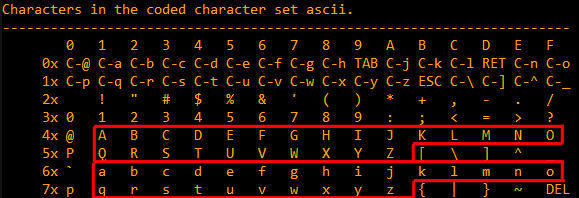
\includegraphics[width=0.7\textwidth]{\CURPATH/ascii.png}
\caption{7-bit \ac{ASCII} table in Emacs}
\end{figure}

\subsection{x64}

\subsubsection{Two comparison operations}

\NonOptimizing MSVC is straightforward: the code checks if the input symbol is in [97..122] range 
(or in [`a'..`z'] range) and subtracts 32 if it's true.

There are also some minor compiler artifact:

\lstinputlisting[caption=\NonOptimizing MSVC 2013 (x64),numbers=left,style=customasm]{\CURPATH/MSVC_2013_x64.asm}

It's important to notice that the input byte is loaded into a 64-bit local stack slot at line 3.

All the remaining bits ([8..63]) are untouched, i.e., contain some random noise (you'll see it in debugger).

% TODO add debugger example
All instructions operate only on byte-level, so it's fine.

The last \TT{MOVZX} instruction at line 15 takes the byte from the local stack slot and zero-extends it to a \Tint 
32-bit data type.

\NonOptimizing GCC does mostly the same:

\lstinputlisting[caption=\NonOptimizing GCC 4.9 (x64),style=customasm]{\CURPATH/GCC_49_x64_O0.s}

\subsubsection{One comparison operation}
\label{toupper_one_comparison}

\Optimizing MSVC does a better job, it generates only one comparison operation:

\lstinputlisting[caption=\Optimizing MSVC 2013 (x64),style=customasm]{\CURPATH/MSVC_2013_Ox_x64.asm}

It was explained earlier how to replace the two comparison operations with a single one: \myref{one_comparison_instead_of_two}.

We will now rewrite this in \CCpp:

\begin{lstlisting}
int tmp=c-97;

if (tmp>25)
        return c;
else
        return c-32;
\end{lstlisting}

The \IT{tmp} variable must be signed.

This makes two subtraction operations in case of a transformation plus one comparison.

In contrast the original algorithm uses two comparison operations plus one subtracting.

\Optimizing GCC is even better, it gets rid of the jumps (which is good: \myref{branch_predictors}) 
by using the CMOVcc instruction:

\lstinputlisting[caption=\Optimizing GCC 4.9 (x64),numbers=left,style=customasm]{\CURPATH/GCC_49_x64_O3.s}

At line 3 the code prepares the subtracted value in advance, as if the conversion will always happen.

At line 5 the subtracted value in EAX is replaced by the untouched input value if a conversion is not needed.
And then this value (of course incorrect) is dropped.

Advance subtracting is a price the compiler pays for the absence of conditional jumps.

\subsection{ARM}

\Optimizing Keil for ARM mode also generates only one comparison:

\lstinputlisting[caption=\OptimizingKeilVI (\ARMMode),style=customasm]{\CURPATH/Keil_ARM_O3.s}

\myindex{ARM!\Instructions!SUBcc}
\myindex{ARM!\Instructions!ANDcc}
The SUBLS and ANDLS instructions are executed only if the value in \Reg{1} is less than 0x19 (or equal).
They also do the actual conversion.

\Optimizing Keil for Thumb mode generates only one comparison operation as well:

\lstinputlisting[caption=\OptimizingKeilVI (\ThumbMode),style=customasm]{\CURPATH/Keil_thumb_O3.s}

\myindex{ARM!\Instructions!LSLS}
\myindex{ARM!\Instructions!LSLR}
The last two LSLS and LSRS instructions work like \TT{AND reg, 0xFF}:
they are equivalent to the \CCpp-expression $(i<<24)>>24$.

Seems like that Keil for Thumb mode deduced that two 2-byte instructions are shorter than the code 
that loads the 0xFF constant into a register plus an AND instruction.

\subsubsection{GCC for ARM64}

\lstinputlisting[caption=\NonOptimizing GCC 4.9 (ARM64),style=customasm]{\CURPATH/GCC_49_ARM64_O0.s}

\lstinputlisting[caption=\Optimizing GCC 4.9 (ARM64),style=customasm]{\CURPATH/GCC_49_ARM64_O3.s}

\subsection{Summary}

All these compiler optimizations are very popular nowadays 
and a practicing reverse engineer usually sees such code patterns often.

